\scanpage{34}

is written, introducing

\margin{\uline{N.B.} $\lambda_\infty\overset{\mathrm{dfn}}{=}-\ell_\infty$}

\[
(6)\qquad
\lambda_\infty\deleted{\unsure{=-\ell_\infty}}
=\rho\sigma\rho^{-1}\sigma\rho
=\rho(\sigma)\sigma\rho
=-\rho\sigma(\rho)^{-1}\rho
=\rho\sigma\rho^{-1}(\sigma)
\]
in the form
\[
(7)\qquad [\sigma,\lambda_\infty]=1.
\]
\margin{N.B. $\sigma=\sigma_\infty$}

\margin{\uline{N.B.} We find
\[
\left\{
\begin{aligned}
[\ell_0,\ell_1]&=[\lambda_0,\lambda_1]=(\sigma(\rho)\rho^{-1})^3\\
[\underbrace{\sigma_{\deleted{\unsure{\infty}}}}_{\sigma}\unsure{,}\ell_\infty]
&=[\underbrace{\sigma_\infty}_{\sigma},\lambda_\infty]
=(\sigma(\rho^{-1})\rho)^3\\
&=\operatorname{int}(\sigma\rho^{-1})\cdot[\ell_0,\ell_1]
\end{aligned}\right.
\]}

We are going to define a group scheme \inserted{$\underline{\mathcal{G}}$} over $\mathbb{Z}$, whose \inserted{$\unsure{\widehat{\mathbb{Z}}|\mathbb{Z}}$-}points will be \inserted{(up to an \unsure{isomorphism} say)} the points of $\widehat{\mathcal{G}}$. We put
\[
(8)\qquad
\underline{M}=\underline{\mathcal{G}}^{\circ}
=\unsure{\mathbb{G}_a|\mathbb{E}_a}^{\{0,1,\infty\}}/\text{diagonal}
\]
\margin{It is better to \unsure{denote} it by $\underline{M}$ --- there are already too many $\mathcal{G}$'s!}

We are going to have \deleted{$\unsure{\mathcal{G}/M}$}
\[
\deleted{(\unsure{4})}(4)\qquad
\mathcal{G}\deleted{\unsure{=\operatorname{GL}(2,\mathbb{Z})}}
\simeq\operatorname{GL}(2,\mathbb{Z})/[\Pi_0,\Pi_0]
\]
operate on $\underline{M}\deleted{\unsure{=\underline{\mathcal{G}}^{\circ}}}$,
\deleted{\unsure{by describing in this way}} \inserted{through}
\[
(5)\qquad
\underbrace{\mathcal{G}_3\times\mu_{\unsure{\tau|2}}^{\deleted{\unsure{2}}}}_{\simeq\unsure{T_{0,3}|\Gamma_{0,3}}}
\simeq\mathcal{G}/M\deleted{\unsure{\widehat{\mathbb{Z}}}}
\simeq\mathcal{G}_{0,3}/\Pi.
\]

Denoting by $\unsure{\overbrace{\dot{\lambda}_0,\dot{\lambda}_1}},\dot{\lambda}_\infty$ the images of the
$\deleted{\lambda_0,\lambda_1}\lambda_i=-\ell_i$ in $\deleted{\unsure{M}}\mathcal{G}$, identified with elements of
\[
M=\mathcal{G}^{\circ}=\underline{\mathcal{G}}^{\circ}(\widehat{\mathbb{Z}})
\]
--- in fact we have
\[
(6)\qquad
\left\{
\begin{aligned}
\dot{\lambda}_0\unsure{,|>}\dot{\lambda}_1,\dot{\lambda}_\infty
&\in\deleted{\unsure{\underline{\mathcal{G}}^{\circ}}}\inserted{\underline{M}}(\mathbb{Z})
\subset\deleted{\unsure{\underline{\mathcal{G}}^{\circ}}}\inserted{\underline{M}}(\widehat{\mathbb{Z}})
=M\otimes_{\unsure{\cdot|\mathbb{Z}}}\unsure{\mathbb{Z}|\widehat{\mathbb{Z}}}\\
\text{thus,}\quad\dot{\lambda}_0+\dot{\lambda}_1+\dot{\lambda}_\infty&=0
\end{aligned}\right.
\]
\margin{(here we write the group law in $M=\underline{\mathcal{G}}^{\circ}$ additively)}

\margin{\figure{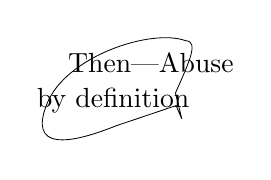
\begin{tikzpicture}[scale=.8]
\draw[line width=.3pt] (1.2,.85) .. controls (.65,1.05) and (-.7,.6) .. (-1,-.15)
 .. controls (-1.3,-.9) and (-.65,-.8) .. (.1,-.5)
 -- (1.05,-.18) -- (1.14,-.39) -- (1.04,.02)
 .. controls (1.25,.5) and (1.42,.84) .. (1.2,.85);
\node at (.65,.5) {\unsure{Then|Abuse}};
\node at (.05,-.1) {by definition};
\end{tikzpicture}}}
$\mathcal{G}_3$ operates on $\underline{M}=\underline{\mathcal{G}}^{\circ}$ by its action on the canonical \deleted{\unsure{bases}} \inserted{generators} $\deleted{\unsure{\lambda_0}}\dot{\lambda}_0,\dot{\lambda}_1,\dot{\lambda}_\infty$, thus
\[
(7)\qquad
\left\{
\begin{aligned}
\sigma(\dot{\lambda}_0)&=\dot{\lambda}_1,\quad
\sigma(\dot{\lambda}_1)=\dot{\lambda}_0
\quad\inserted{\text{hence}}\quad
\sigma(\dot{\lambda}_\infty)=\dot{\lambda}_\infty\\
\rho(\dot{\lambda}_i)&=\dot{\lambda}_{i+1}
\end{aligned}\right.
\]
\margin{This is seen first for $i=0,1$ and, \unsure{is deduced from it} for $i=\infty$.}
On the other hand we have by definition
\[
(8)\qquad\tau(\dot{\lambda}_i)=-\dot{\lambda}_i
\]
where
\diagram{\begin{tikzcd}[column sep=2pt,row sep=small]
\tau\arrow[d,equal]&{}={}&\sigma&\tau'\arrow[d,equal]\\
\tau_\infty&&&\tau'_\infty
\end{tikzcd}}

\margin{33}

\scanpage{35}
\mspage{665}

. The announced extension $\underline{\mathcal G}$ is of course that of § 50 3°), \unsure{developed} in the meantime (since the first lines of the present §, noting precisely that I was feeling cramped in making the construction explicit) :

(9)\quad\diagram{\begin{tikzcd}[column sep=large]
1 \arrow[r] & \underline M \arrow[r] \arrow[d,equal] & \underline{\mathcal G} \arrow[r] & H_{S_0} \arrow[r,no head] & 1 \\
 & \check V(M) & & &
\end{tikzcd}}
where $S_0=\operatorname{Spec}\mathbb Z$.

For $\unsure{\forall}$ scheme $S$, we will put
\[
\tag{10}
\begin{gathered}
\underline{\mathcal G}^{\Delta}(S)\subset\underline{\mathcal G}(S)\\
\Vert\;\mathrm{dfn}\\
\text{Inverse image of the ``diagonal'' of}\\
\Gamma(H_{\unsure{S|S_0}}/S)
\quad\bigl(\text{i.e. of the image of }H\longrightarrow\Gamma(H_{\unsure{S|S_0}},S)\bigr)\\
\text{under the canonical homomorphism }\underline{\unsure{\mathcal G|\mathcal E}}(S)\longrightarrow H_S(S),
\end{gathered}
\]
so that by the construction of loc. cit. we will have a canonical isomorphism
\[
\tag{11}
\underline{\mathcal G}^{\Delta}(S)\simeq
\mathcal G\underset{M}{\wedge}\deleted{\unsure{A}}
\underbrace{\Gamma(S,\underline{\mathcal O}_S\otimes_{\mathbb Z}M)}_{
\simeq\deleted{\unsure{A}}\inserted{M}\otimes_{\mathbb Z}A\ \text{if}}
\]
and a canonical exact sequence

(12)\quad\diagram{\begin{tikzcd}[column sep=large]
1 \arrow[r] & \underbrace{\Gamma(S,\underline{\mathcal O}_S\otimes_{\mathbb Z}M)}_{A\otimes_{\mathbb Z}M} \arrow[r] & \underline{\mathcal G}^{\Delta}(S) \arrow[r] & H \arrow[r] & 1.
\end{tikzcd}}

\figure{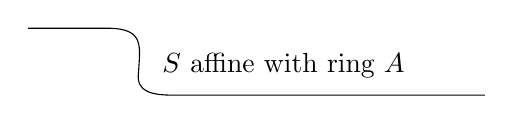
\begin{tikzpicture}[x=1cm,y=1cm]
\draw (0,0.75) -- (1.0,0.75)
.. controls (1.48,0.75) and (1.42,0.53) .. (1.40,0.18)
.. controls (1.37,-0.06) and (1.57,-0.10) .. (1.85,-0.10)
-- (5.80,-0.10);
\node[anchor=west] at (1.58,0.28) {$S$ affine with ring $A$};
\end{tikzpicture}}

Taking $A=\widehat{\mathbb Z}$, we find in particular (and this is again a general fact about group schemes associated with extensions of discrete groups with abelian kernel)
\[
\tag{13}
\mathcal G^{\wedge}\simeq\underline{\mathcal G}^{\Delta}(\widehat{\mathbb Z}).
\]
\margin{34}

\scanpage{36}

2. The group $\widetilde Z_{\rho,\sigma}$ : \uline{provisional version}.

. I am now going to make explicit for $\widehat{\mathcal G}$ and $\widehat{\mathcal G}_{\unsure{0|\bullet}}\longrightarrow\widehat{\mathcal G}$ the general constructions of § 49 $\overline{\underline{\mathrm{VI}}}$, taking \inserted{there} \deleted{$\unsure{\mathcal G}$}
\[
\tag{14}
\underline{\mathcal G}^{\unsure{\natural}}\overset{\mathrm{dfn}}=
\underline M=\underline{\mathcal G}^{\circ}
\quad(\text{identity component of }\underline{\mathcal G})
\]
In a case like this one, where $\underline{\mathcal G}^{\unsure{\natural}}$ is precisely the closed subgroup of the $(\rho,\sigma)$-group $\mathcal G_{\rho,\sigma}$ $(=\mathcal G^{\wedge}\text{ here})$ generated by $\lambda_0,\lambda_1,\lambda_\infty$, we \unsure{will dispense} in the notation --- where there is no ambiguity --- with including the notation $\unsure{\natural}$. For \unsure{$\forall$ $A$} we will have to distinguish for example between $G_{\rho,\sigma}$ and $G_{\rho,\sigma}^{\unsure{\natural}}$ etc. \uline{We will however carry out the constructions in the scheme-theoretic setting, rather than the profinite one.}

\margin{I think I will compare the two possible constructions at the end. The \unsure{underlines} will indicate the group \uline{schemes}...}

The essential step is to determine the group $\underline Z_{\rho,\sigma}$
\[
\tag{15}
\begin{gathered}
\underline Z_{\rho,\sigma}\subset\underline{\operatorname{Aut}}(\underline{\mathcal G}^{+})\\
\Vert\;\mathrm{dfn}\\
\left\{u\in\underline{\operatorname{Aut}}(\mathcal G^{+})\ \left|\
\begin{aligned}
\deleted{\unsure{1^{\circ}}}\ \text{a)}\;&\exists\alpha\in\underline{\mathcal G}_{\tau}^{\unsure{\natural}}=\{1,\tau\}.\underline M,
&&u(\rho)=\alpha(\rho)\\
\text{b)}\;&\exists\beta\in\text{-- -- -- -- -- --}
&&u(\sigma)=\beta(\sigma)\\
\text{c)}\;&u(L_0^{\deleted{\unsure{\Pi_0}}\mathcal G})=L_0^{\mathcal G}
&&\deleted{\unsure{(\Longleftrightarrow L_0^{\Pi_0}=L_0^{\natural})}}\\
&\qquad(\Longleftrightarrow u(L_0^{\Pi_0})=L_0^{\Pi_0})\\
\bigl[\text{d)}\;&(\text{automatic})\quad u(\mathcal G^{\unsure{\natural}})\subset\mathcal G^{\unsure{\natural}}\bigr]
\end{aligned}\right.\right.
\end{gathered}
\]

\margin{here, ``$\exists\alpha$'' ``$\exists\beta$'' of course means the \uline{local} existence of $\alpha,\beta$...}

Let us note that $u$ is determined by the values
\[
\tag{16}
\begin{cases}
u(\rho)=\xi\rho\\
u(\sigma)=\eta\sigma
\end{cases}
\qquad\xi,\eta\in\Gamma\underline\Pi
\]
\margin{where $\underline\Pi=\underline M\unsure{\rtimes}\deleted{\unsure{\{1,\tau\}}}\inserted{\unsure{\mu_2}}$ ($\underline M$ \unsure{subgroup|is a group} of index $2$ in $\underline\Pi$)}
\inserted{$\xi,\eta$} satisfying the following conditions ;
\margin{35}

\scanpage{37}
\mspage{666}

\[
\tag{17}
\left\{
\begin{aligned}
\text{a)}\;&\xi\rho\ \text{(locally) conjugate to }\rho\ \text{via }\underline{\unsure{\mathcal G}}^{\unsure{\natural}}=\underline M\\
\text{b)}\;&\eta\sigma\ \text{-- -- -- -- -- -- ---}\ \sigma\ \text{'' -- -- ---}\\
\text{c)}\;&\text{loop equation}\\
&\xi=\eta\ell_1^{\nu}\quad\text{where }\nu\in\Gamma\mathbb G_a\ \text{suitable}\\
&\qquad\bigl(\text{such that }\mu\overset{\mathrm{dfn}}=2\nu+1\in\Gamma\mathbb G_m\bigr)
\end{aligned}\right.
\]

. \deleted{Since $\xi,\eta\in\Gamma N$, it will be necessary}

\uline{Remark} It is no longer possible here to denote by $-1$ the nontrivial element \inserted{$\omega$} of the center $\unsure{\mu|\mu_2}$ of $\mathcal G^{\wedge}$, and to denote by $-x$ (for $x\in\mathcal G^{\wedge}$) the product of $x$ with it, because of the confusion with the notation $-x$ \inserted{(for $x\in M$)} in the abelian group $M$ for the inverse of $x$ --- but \deleted{\unsure{the element}} $\omega x\ne-x$, since $\omega x\notin M$, $-x\in M$...

We of course put
\[
\tag{18}
\varepsilon_3(u)=\varepsilon_{\mathcal G}(\alpha),\qquad
\varepsilon_2(u)=\varepsilon_{\mathcal G}(\beta)
\]
(well defined, since $\rho$ and $\rho^{-1}$ are not conjugate on any fiber, idem for $\sigma,\sigma^{-1}$), how to make them explicit in terms of $\xi,\eta$ ? We will have

\deleted{\unsure{(17)}}
\[
\tag{19}
\left\{
\begin{aligned}
\xi=\alpha\rho(\alpha)^{-1}
&\left\{
\begin{aligned}
&\in\Gamma\underline M\quad\text{if }\alpha\in\Gamma\underline M=\Gamma\underline{\mathcal G}^{\unsure{\natural}}\ \text{i.e. }\varepsilon_3(u)=1\\
&=\underbrace{\alpha_0}_{\in\Gamma\underline M}\tau\rho(\alpha_0\tau)^{-1}
=\alpha_0\underbrace{(-\ell_1^{-1})}_{\lambda_1^{-1}\in\underline M}\rho(\alpha_0)^{-1}\in\Gamma\underline M\quad\text{if }\varepsilon_3(u)=\unsure{-1}
\end{aligned}\right.\\[1ex]
\eta=\beta\sigma(\beta)^{-1}
&\left\{
\begin{aligned}
&\in\Gamma\underline M\quad\text{if }\beta\in\Gamma\underline M=\Gamma\underline{\mathcal G}^{\unsure{\natural}}\ \text{i.e. }\varepsilon_2(u)=1\\
&=(\underbrace{\beta_0}_{\in\Gamma\underline M}\tau)\sigma(\beta_0\tau)^{-1}
=\omega\beta_0\sigma(\beta_0)^{-1}\in\omega\underline M\quad\text{if }\varepsilon_2(u)=\unsure{-1}
\end{aligned}\right.
\end{aligned}\right.
\]
thus in any case
\[
\tag{19 bis}
\begin{cases}
\xi\in\Gamma\underline M\\
\eta\in\Gamma\bigl(\omega^{\nu_2(u)}.\underline{M}\bigr)
\end{cases}
\]
\margin{36}

\scanpage{38}
\mspage{676}

from which we get, by the loop equation (17)
\[
\tag{20}
\ell_1^{\nu}=(\omega\lambda_1)^{\nu}\in\Gamma(\omega^{\nu_2(u)}.\underline M)
\quad\text{i.e. }\unsure{\Longleftrightarrow}\ \omega^{\nu}\in\Gamma(\omega^{\nu_2(u)}.\underline M)
\]
We can write it in the form
\[
\tag{21}
\underline\nu=2\underline\nu'+\underline\nu_2
\]
where
\[
\tag{22}
\left\{
\begin{aligned}
\underline\nu,\underline\nu' &: Z_{\rho,\sigma}\longrightarrow\mathbb G_a\\
\underline\nu_2,\underline\nu_3 &: Z_{\rho,\sigma}\rightrightarrows
(\mathbb Z/2\mathbb Z)_{S_0}^{\unsure{\mathrm{que}|\mathrm{cste}}}
\end{aligned}\right.
\]
\deleted{$\unsure{\varepsilon}$}
are well-defined \unsure{morphisms} of schemes, related \inserted{to one another and} to the group homomorphisms \deleted{$\unsure{\mu}$}
\[
\underline\mu:Z_{\rho,\sigma}\longrightarrow\mathbb G_m,\qquad
\underline\varepsilon_{\unsure{1|2}},\underline\varepsilon_3:Z_{\rho,\sigma}\longrightarrow\{\pm1\}_{S_0}
\]
by the formulas (21) and
\[
\tag{23}
\left\{
\begin{aligned}
\underline\mu&=2\underline\nu\,\unsure{+}\,1\deleted{\unsure{+1}}
\quad(=4\underline\nu'\,\unsure{+}\,2\underline\nu_2+1)\\
\underline\varepsilon_2&=(-1)^{\underline\nu_2},\qquad
\underline\varepsilon_3=(-1)^{\underline\nu_3}.
\end{aligned}\right.
\]

We will therefore have, by virtue of (\unsure{24|21})
\deleted{
\[
\tag{24}
\ell_1^{\nu}=\ell_1^{2\nu'}\ell_1^{\nu_2}
=\underbrace{(\omega\lambda_1)}_{\lambda_1}^{2\nu'}\ell_1^{\nu_2}
=\lambda_1^{2\nu'}\ell_1^{\nu_2}
\]
Since $\ell_1=\lambda_1\omega$, we
\deleted{I feel like putting the $\ell_i$ in the form}
\[
\tag{25}
\ell_i=a_i\omega\quad\text{where }a_i\in\underline M!
\]
can \deleted{\unsure{to thus|will be able to}} write (24) in the form
\[
\tag{26}
\ell_1^{\nu}=\underbrace{(\lambda_1^{\unsure{2\nu'}}a_1^{\nu_2})}_{\in\Gamma\underline M}\omega^{\nu_2}
\quad\deleted{\text{for }\unsure{\nu_2=0|\nu_2=1}\ \text{i.e. }\unsure{\varepsilon_2=1}}
\]
To make the $a_i$ explicit, we must expand them as linear combinations of $\lambda_0,\lambda_1,\lambda_\infty$ (or of two of them, if we want uniqueness).
}
\margin{37}